%%% template.tex
%%% This is a template for making up an AMS-LaTeX file
%%% Version of February 12, 2011
%%%---------------------------------------------------------
%%% The following command chooses the default 10 point type.
%%% To choose 12 point, change it to
%%% \documentclass[12pt]{amsart}
\documentclass{amsart}
\usepackage{cite}
%%% The following command loads the amsrefs package, which will be
%%% used to create the bibliography:
\usepackage[lite]{amsrefs}

% personal macros
\usepackage{macros}


\usepackage{hyperref}
\hypersetup{
    colorlinks,
    citecolor=black,
    filecolor=black,
    linkcolor=black,
    urlcolor=black
}

\usepackage{parskip} % Automatically respects blank lines
\setlength{\parskip}{1em} % Adds more space between paragraphs
\setlength{\parindent}{0pt} % Removes paragraph indentation

\makeatletter
\renewcommand{\l@section}{\@tocline{1}{-6pt}{1.5em}{2.3em}{}}
\renewcommand{\l@subsection}{\@tocline{2}{-6pt}{3.8em}{3.2em}{}}
\renewcommand{\l@subsubsection}{\@tocline{3}{-6pt}{7.0em}{4.1em}{}}
\makeatother


%%% The following command defines the standard names for all of the
%%% special symbols in the AMSfonts package, listed in
%%% http://www.ctan.org/tex-archive/info/symbols/math/symbols.pdf
\usepackage{amssymb}
\usepackage{tikz-cd}
\usetikzlibrary{decorations.pathmorphing}
\usepackage{float}



%%% The following commands allow you to use \Xy-pic to draw
%%% commutative diagrams.  (You can omit the second line if you want
%%% the default style of the nodes to be \textstyle.)
\usepackage[all,cmtip]{xy}
\let\objectstyle=\displaystyle

%%% If you'll be importing any graphics, uncomment the following
%%% line.  (Note: The spelling is correct; the package graphicx.sty is
%%% the updated version of the older graphics.sty.)
% \usepackage{graphicx}

%%% This part of the file (after the \documentclass command,
%%% but before the \begin{document}) is called the ``preamble''.
%%% This is where we put our macro definitions.

%%% Comment out (or delete) any of these that you don't want to use.

%%%-------------------------------------------------------------------
%%%-------------------------------------------------------------------
%%% The Theorem environments:
%%%
%%%
%%% The following commands set it up so that:
%%% 
%%% All Theorems, Corollaries, Lemmas, Propositions, Definitions,
%%% Remarks, Examples, Notations, and Terminologies  will be numbered
%%% in a single sequence, and the numbering will be within each
%%% section.  Displayed equations will be numbered in the same
%%% sequence. 
%%% 
%%% 
%%% Theorems, Propositions, Lemmas, and Corollaries will have the most
%%% formal typesetting.
%%% 
%%% Definitions will have the next level of formality.
%%% 
%%% Remarks, Examples, Notations, and Terminologies will be the least
%%% formal.
%%% 
%%% Theorem:
%%% \begin{thm}
%%% 
%%% \end{thm}
%%% 
%%% Corollary:
%%% \begin{cor}
%%% 
%%% \end{cor}
%%% 
%%% Lemma:
%%% \begin{lem}
%%% 
%%% \end{lem}
%%% 
%%% Proposition:
%%% \begin{prop}
%%% 
%%% \end{prop}
%%% 
%%% Definition:
%%% \begin{defn}
%%% 
%%% \end{defn}
%%% 
%%% Remark:
%%% \begin{rem}
%%% 
%%% \end{rem}
%%% 
%%% Example:
%%% \begin{ex}
%%% 
%%% \end{ex}
%%% 
%%% Notation:
%%% \begin{notation}
%%% 
%%% \end{notation}
%%% 
%%% Terminology:
%%% \begin{terminology}
%%% 
%%% \end{terminology}
%%% 
%%%       Theorem environments

% The following causes equations to be numbered within sections
\numberwithin{equation}{section}


% We'll use the equation counter for all our theorem environments, so
% that everything will be numbered in the same sequence.

%       Theorem environments

\theoremstyle{plain} %% This is the default, anyway
\newtheorem{theorem}[equation]{Theorem}
\newtheorem{cor}[equation]{Corollary}
\newtheorem{lemma}[equation]{Lemma}
\newtheorem{proposition}[equation]{Proposition}

\theoremstyle{definition}
\newtheorem{definition}[equation]{Definition}

\theoremstyle{remark}
\newtheorem{remark}[equation]{Remark}
\newtheorem{example}[equation]{Example}
\newtheorem{notation}[equation]{Notation}
\newtheorem{terminology}[equation]{Terminology}

%%%-------------------------------------------------------------------
%%%-------------------------------------------------------------------
%%%-------------------------------------------------------------------
%%%-------------------------------------------------------------------
%%%-------------------------------------------------------------------
%%%-------------------------------------------------------------------
%%%-------------------------------------------------------------------
\begin{document}

%%% In the title, use a double backslash "\\" to show a linebreak:
%%% Use one of the following two forms:
%%% \title{Text of the title}
%%% or
%%% \title[Short form for the running head]{Text of the title}
\title{Moment maps and equivariant cohomology in toric geometry}


%%% If there are multiple authors, they're described one at a time:
%%% First author: \author{} \address{} \curraddr{} \email{} \thanks{}
%%% Second author: \author{} \address{} \curraddr{} \email{} \thanks{}
%%% Third author: \author{} \address{} \curraddr{} \email{} \thanks{}
\author{Songyu Ye} \email{sy459@cornell.edu}

%%% In the address, show linebreaks with double backslashes:
\address{}

%%% Current address is optional.
% \curraddr{}

%%% Email address is optional.
% \email{}


%%% If there's a second author:
% \author{}
% \address{}
% \curraddr{}
% \email{}


%%% To have the current date inserted, use \date{\today}:
\date{\today}

%%% To include an abstract, uncomment the following two lines and type
%%% the abstract in between them:
\begin{abstract}
    Toric varieties serve as a rich interface between algebraic geometry, symplectic geometry, and combinatorics. Their structure is deeply tied to combinatorial objects such as polytopes and fans, which encode their topology and geometry. This thesis explores the construction of toric varieties via moment maps, symplectic reduction, and Geometric Invariant Theory, providing a comprehensive framework for understanding these spaces. The central focus is the application of equivariant cohomology, a refinement of ordinary cohomology, which captures additional symmetries and enriches the topological study of toric varieties. We utilize combinatorial techniques, including localization formulas, shellings, and the Białynicki-Birula decomposition, to analyze the topology and cohomological invariants of these varieties. 
\end{abstract}


\maketitle
\tableofcontents


%%%-------------------------------------------------------------------
%%%-------------------------------------------------------------------
%%% Start the body of the paper here!  E.G., maybe use:
%%% \section{Introduction}
%%% \label{sec:intro}

%%% For a numbered display, use
%%% \begin{equation}
%%%   \label{something}
%%%   The display goes here
%%% \end{equation}
%%% and you can refer to it as \eqref{something}.

%%% For an unnumbered display, use
% \begin{equation*}

% \end{equation*}

%%% To import a graphics file, you must have said
%%% \usepackage{graphicx}
%%% in the preamble (i.e., before the \begin{document}).
%%% Putting it into a figure environment enables it to float to the
%%% next page if there isn't enough room for it on the current page.
%%% The \label command must come after the \caption command.
% \begin{figure}[h]
%   \includegraphics{filename}
%   \caption{Some caption}
%   \label{somelabel}
% \end{figure}

\section{Introduction}
Toric varieties are a fundamental class of spaces in algebraic geometry, characterized by their combinatorial and geometric simplicity. They arise naturally in several mathematical disciplines, including symplectic geometry, representation theory, and mathematical physics, see \cite{cannas} and \cite{oda}. They also provide, as Fulton writes in \cite{fulton}, “a remarkably fertile testing ground for general theories.”

In this work, we begin by describing several polytopal constructions that highlight the interplay between algebraic and symplectic geometry, showcasing the fluid transitions between these two perspectives. We then introduce the concept of fans, which provide an equivariant atlas of charts for abstract toric varieties. These combinatorial tools offer a powerful framework for understanding the topology of toric varieties, enabling precise calculations and interpretations. Using these combinatorial insights, we investigate the equivariant cohomology of toric varieties. 

As a refinement of ordinary cohomology, equivariant cohomology captures additional symmetries and provides a richer topological invariant. A unique feature of equivariant cohomology is the localization package for equivariantly formal spaces, developed by Atiyah-Bott and Berline-Vergne. We study the localization formula and the GKM conditions, which are central tools in the analysis of toric varieties. In particular, we introduce the Bialynicki-Birula decomposition, an algebraic analogue of Morse theory, and demonstrate that smooth projective toric varieties are equivariantly formal.


\section{Constructing toric varieties}
We describe multiple equivalent constructions of a toric variety starting from the data
of a polytope $P$ subject to certain conditions. Each of 
the constructions will yield us a space $X_i(P)$ which will all be 
equivariantly diffeomorphic to each other as smooth manifolds. 


% Depending on the nature of the construction, $X_i(P)$ will either be 
% a projective toric variety or a toric symplectic manifold, and these 
% two classes of spaces can be identified with each other via the image 
% of their moment maps.



\subsection{Delzant polytopes}
Let $V$ be a real vector space of dimension $n$ and let $V_\Z$
be a lattice inside $V$. Given 
$N$ linear functionals $a_i \in V^*$ preserving $V_\Z$ and $N$ integers $\lambda_i$
the set \begin{align*}
P = \{ v \in V \mid a_i(v) + \lambda_i \geq 0 \text{ for all } i \}.
\end{align*} is called a \emph{rational polyhedron}. It is called 
a \emph{rational polytope} if it is bounded. We will assume that $P$ is a
rational polytope throughout this paper. A polytope $P$ has \emph{facets} \begin{align*}
F_i = \{ v \in P \mid a_i(v) + \lambda_i = 0 \}
\end{align*} and \emph{faces} which are intersections of facets. 
The \emph{vertices} of $P$ are the 0-dimensional faces of $P$ and 
the \emph{edges} of $P$ are the 1-dimensional faces of $P$.
We say $P$ is: \begin{itemize}
    \item \emph{simple} if exactly $n$ edges meet at each vertex
    \item \emph{smooth} if the edges meeting at each vertex form a basis for $V_\Z$
    \item \emph{Delzant} if $P$ is simple and smooth
\end{itemize}

\begin{example}
    The right triangle $P = \{ (x,y) \in \R^2 \mid x \geq 0, y \geq 0, x + y \leq 1 \}$ is a 
    Delzant polytope. The standard tetrahedron $P\subset\R^3$ is not Delzant because the
    top vertex is not simple.
\end{example}
We begin by stating the correspondence we are interested in.
\begin{theorem}\label{thm:delzant}
    [Delzant] There is a correspondence between Delzant polytopes up to $\GL(n,\Z)$ 
    and translation, and toric symplectic manifolds up to equivariant symplectomorphism.
\end{theorem}

\begin{theorem}
    There is a correspondence between Delzant polytopes up to $\GL(n,\Z)$
    and translation, and smooth projective toric varieties with a particular choice
    of very ample line bundle, up to equivariant isomorphism.
\end{theorem}

\subsection{Moment maps}
Let $(M,\omega)$ be a symplectic manifold. The nondegeneracy of $\omega$ allows us to
pair vector fields with 1-forms. We say that a vector field $X$ is \emph{Hamiltonian} if
the corresponding 1-form $\iota_X\omega = \omega(X,\cdot)$ is exact, in which case 
it is equal to $dH$ for some smooth function $H$. The function $H$ is called a
\emph{Hamiltonian} of $X$. 

\hfill

Given a Lie group $G$ acting on $M$ by symplectomorphisms,
the Lie algebra $\mathfrak{g}$ acts on $M$ by symplectic vector fields.
This linearized action of $\mf g$ is given by the expression
\begin{align*}
    X_\zeta(m) = \frac{d}{dt}\Big|_{t=0} \exp(t\zeta)\cdot m
\end{align*} where we interpret the given expression via parallel transport along the flow of $\zeta$.

\begin{remark}
    In general, whenever we have a Lie group $G$ acting on a manifold $M$, we get a linearized
    action of $\mf g$ on $\Gamma(E)$ for any vector bundle $E$ over $M$. For the trivial 
    line bundle $E = M\times \R$ we have $\Gamma(E) = C^\infty(M)$ and the linearized action
    of $\mf g$ on $C^\infty(M)$ is given by the Lie derivative of 
    the function along the vector field.
\end{remark}

\begin{example}
    Consider $G = \SL(2,\C)$ acting on $\P^1$ by linear fractional transformations. Explicitly
    we have \begin{align*}
        \begin{pmatrix}
            a & b \\
            c & d
        \end{pmatrix} \cdot [z_0:z_1] = [az_0 + bz_1 : cz_0 + dz_1]
    \end{align*} The Lie algebra $\mf{sl}(2,\C)$ is generated by the matrices \begin{align*}
        E = \begin{pmatrix}
            0 & 1 \\
            0 & 0
        \end{pmatrix} \quad F = \begin{pmatrix}
            0 & 0 \\
            1 & 0
        \end{pmatrix} \quad H = \begin{pmatrix}
            1 & 0 \\
            0 & -1
        \end{pmatrix}
    \end{align*} Writing down the exponential, we find that \begin{align*}
        \exp(tE) = I + tE \quad \text{since } E^2 = 0
        \implies \exp(tE)\cdot [z_0:z_1] = [z_0 + tz_1 : z_1]
    \end{align*} On an affine chart, the action of $E$ is given by $z \mapsto z + t$ and
    we compute \begin{align*}
        \frac{d}{dt}\Big|_{t=0} z + t = 1 \implies X_E(z) = \frac{\partial}{\partial z}
    \end{align*} Similarly we compute \begin{align*}
        \exp(tH) = \begin{pmatrix}
            e^t & 0 \\
            0 & e^{-t}
        \end{pmatrix} \implies \exp(tH)\cdot [z_0:z_1] = [e^tz_0 : e^{-t}z_1]
    \end{align*} which looks like $z\mapsto e^{2t}z$ on an affine chart, which gives us
     \begin{align*}
        \frac{d}{dt}\Big|_{t=0} e^{2t}z = 2z \implies X_H(z) = 2z \frac{\partial}{\partial z}
    \end{align*} Finally we compute \begin{align*}
        \exp(tF) = 1 + tF \implies \exp(tF)\cdot [z_0:z_1] = [z_0 : z_1 + tz_0]
    \end{align*} On an affine chart this transformation looks like $z\mapsto z/(1+tz)$
    and we compute \begin{align*}
        \frac{d}{dt}\Big|_{t=0} \frac{z}{1+tz} = -z^2 \implies X_F(z) = -z^2\frac{\partial}{\partial z}
    \end{align*} In particular we get a map $\mf{sl}(2,\C) \to \Gamma(T\P^1)$ given by
    \begin{align*}
        E &\mapsto \frac{\partial}{\partial z} \\
        H &\mapsto 2z\frac{\partial}{\partial z} \\
        F &\mapsto -z^2\frac{\partial}{\partial z}
    \end{align*} which is the standard action of $\mf{sl}(2,\C)$ on $T\P^1$. This map in fact 
    extends to an isomorphism between the enveloping algebra $U(\mf{sl}(2,\C))$ and 
    the algebra of differential operators on $\cD_{\text{hol}}(\P^1)$. This is a 
    shadow of the Beilinson-Bernstein localization theorem (cf. \cite{htt}).
\end{example}

We say that the
action of $G$ is \emph{weakly Hamiltonian} 
if for every $\zeta\in\mf g$ the corresponding vector field $X_\zeta$ is Hamiltonian,
i.e. $\iota_{X_\zeta}\omega = dH_\zeta$ for some smooth function $H_\zeta$. The $H_\zeta$
is determined only up to a constant, so choose the map $\mf g \to C^\infty(M)$ given by 
$\zeta \mapsto H_\zeta$ to be linear. If the map can be chosen to be equivariant with respect
to the adjoint action of $G$ on $\mf g$, then the action of $G$ is called \emph{Hamiltonian}.
In this case, there is a map $\mu : M \to \mf g^*$ called the \emph{moment map} defined by
\begin{align*}
    H_\zeta(m) := \langle \mu(m), \zeta \rangle
\end{align*}
If the action of $G$ is Hamiltonian, then the moment map is $G$-equivariant and unique up 
to the addition of a constant. When $G = T$ is a torus, the adjoint action 
is trivial and the moment map $\mu : M \to \mf t^*$
is $T$-invariant.

\begin{theorem}\label{thm:ags}
    [Atiyah-Guillemin-Sternberg Convexity Theorem] Let $M$ be a compact connected symplectic manifold with a
    Hamiltonian $T$-action. Then the image of the moment map is a convex polytope 
    in $\mf t^*$ whose vertices are the image of the fixed points of the $T$-action.
\end{theorem}
\begin{proof}
    See \cite{mcduff-salamon}.
\end{proof}

We say $M$ is a \emph{toric symplectic manifold} in the sense of Theorem \ref{thm:delzant}
if $(M,\omega)$ is a compact connected symplectic manifold
with a effective (meaning no element of $T$ acts trivially) Hamiltonian $T$-action.

\begin{proposition}
    Let $M\subset \C\P^n$ be a smooth projective toric variety embedded by a line bundle.
    Then $M$ is equivariantly symplectomorphic to a toric symplectic manifold.
\end{proposition}
\begin{proof}
$\C\P^n$ carries a natural symplectic form $\omega$ 
called the Fubini-Study form. Any smooth projective toric variety $M$ embedded
in projective space carries a symplectic form $\omega$ induced by pulling 
back the Fubini-Study form. Moreover, the action of $T$ on $M$
 is Hamiltonian with respect to $\omega$.
\end{proof}

\hfill

Conversely, given a toric symplectic manifold $(M,\omega)$, we can associate a 
smooth projective toric variety to the moment polytope $\mu(M)$ which will be
equivariantly symplectomorphic to $M$.

\subsection{Symplectic reduction}
We describe how to construct $M$ as the symplectic reduction of affine space $\C^N$ for 
a particular moment map. In particular, $M$ carries a natural symplectic form $\omega$ and 
a Hamiltonian $T$-action.
This section follows \cite{lsg}. 

\hfill 

Let $P$ be a Delzant polytope.
There are maps \begin{align*}
    \pi:\R^N&\to\R^n\\
    e_i &\mapsto a_i
\end{align*} and the induced map \begin{align*}
    \pi: \R^N/\Z^N\to\R^n/\Z^n 
\end{align*} of tori, which give rise to the following short exact sequences. \begin{align}\label{eq:ses1}
    1\to K \to \T^N \to \T^n \to 1
\end{align} \begin{align*}
    0\to k \to \R^N\to \R^n\to 0
\end{align*} The dual of the second sequence gives \begin{align*}
    0 \to (\R^n)^* \to (\R^N)^* \to k^* \to 0
\end{align*} and denote the map $i^* : (\R^N)^*\to k^*$. Now consider $\C^N$
with the standard symplectic form $\omega = \sum dz_i\wedge d\bar z_i$ and the 
standard Hamiltonian torus action \begin{align*}
    (e^{i\theta_1},\dots,e^{i\theta_N})\cdot(z_1,\dots,z_N) = (e^{i\theta_1}z_1,\dots,e^{i\theta_N}z_N)
\end{align*} and corresponding moment map \begin{align*}
    \phi:\C^N&\to(\R^N)^* \\
    \phi(z_1,\dots,z_N) &= -\pi(|z_1|^2,\dots,|z_N|^2) + (\lambda_1,\dots,\lambda_N)
\end{align*}
The subtorus $K$ acts on $\C^N$ via restriction and the restricted action is 
Hamiltonian. Moreover, the moment map for the action of $K$ is given by $i^*\circ\phi:M\to k^*$.

\hfill

Let $Z = (i*^\circ \phi)^{-1}(0)$ be the zero level set of the moment map. The following 
claims are all justified in \cite{lsg}.

\begin{lemma}
    $Z$ is compact and $K$ freely acts on $Z$. 
\end{lemma}

The following theorem tells us that the orbit space $Z/K$ is a symplectic manifold.

\begin{theorem}{\label{thm:reduction}}
    [Marsden-Weinstein-Meyer] Let $G$ be a compact group and let $(M,\omega)$ be a symplectic manifold with a
    Hamiltonian $G$-action. Let $i:\mu^{-1}(0)\to M$ be the inclusion of the zero level set of the moment map.
    Assume $G$ acts freely on $\mu^{-1}(0)$. Then \begin{itemize}
        \item the orbit space $M_{\text{red}} = \mu^{-1}(0)/G$ is a smooth manifold
        \item $\pi:\mu^{-1}(0)\to M_{\text{red}}$ is a principal $G$-bundle
        \item there is a unique symplectic form $\omega_{\text{red}}$ on $M_{\text{red}}$ such that $\pi^*\omega_{\text{red}} = i^*\omega$
    \end{itemize}
\end{theorem}
Symplectic reduction realizes one direction of Delzant's correspondence.
\begin{proposition}
    The reduced space $X_1(P) := Z/K$ is a toric symplectic manifold with moment map image $P$.
\end{proposition}

\subsection{Monoid algebra}
Let $P$ be a Delzant polytope. Consider the cone \begin{align*}
    \sigma_P = \{ (v,t) \in V \times \R \mid v \in tP, t \geq 0 \}
\end{align*} The lattice points of this cone 
form a semigroup $S_P$. Define the space \begin{align*}
    X_2(P) = \Proj \C[S_P]
\end{align*} 

\begin{proposition}
    The space $X_2(P)$ is a smooth projective toric variety.
\end{proposition}
This follows from general theory of projective toric varieties. We 
refer the reader to chapter 2 of \cite{cls} for a detailed exposition.

\subsection{Projective GIT}
Let $P$ be a Delzant polytope. Complexifying (\ref{eq:ses1}), we get \begin{align*}
    1\to K_\C \to T_\C^N \to T_\C^n \to 1 
\end{align*} Let $F_i$ denote the facets of $\Delta$ and for any $z = (z_1,\dots,z_N)\in\C^n$ let $F_z := \cap_{z_i = 0}F_i$.
Consider the set \begin{align*}
    U = \{z\in\C^n: F_z \neq \emptyset\}
\end{align*} Then the quotient $X_3(P) = U/K_\C$ is a manifold with an action of $T_\C^N/K_\C = T_\C^n$. It 
is a smooth projective toric variety \red{because it is a projective GIT quotient}.

\begin{remark}
    There is a surjective map from $X^{ss}$ to $X//G$. Two points in $X^{ss}$ lie in the same fiber of this map if and only if the closures of their 
    $G$-orbits intersect. In this case, the $K_\C$ orbits are closed. See \cite{proudfoot} for more details.
\end{remark}
\subsection{Kempf-Ness theorem}
We want to compare the symplectic quotient to the projective GIT quotient.  First recall
that if $K$ is a real compact group, then its complexification $G := K_\C$ is a 
complex Lie group which contains $K$ and $\mf g = \mf k \oplus i\mf k$ is the complexification
 of $\mf k$. See \cite{hoskins} for more details about the following theorems.

\begin{theorem}
    Complexification defines a bijection between the isomorphism
    classes of compact real Lie groups and complex reductive groups.
\end{theorem}
The following theorem of Kempf-Ness states a relationship between the symplectic quotient and the GIT quotient.
\begin{theorem}{\label{thm:kempf-ness}}
    [Kempf-Ness] 
    Let $G$ be a complex reductive group acting on a smooth complex projective variety 
    $X\subset \P^n$. Let $K$ be a maximal compact subgroup of $G$ and suppose $K$ 
    is connected and acts on $X$ Hamiltonianly. Let $\mu:X\to\mf k^*$ be the moment map. 
    Then the inclusion $\mu^{-1}(0)\to X$ induces a homeomorphism \begin{align*}
        \mu^{-1}(0)/K \to X//G
    \end{align*}
\end{theorem}

\begin{remark}
    \red{We should say more about this theorem}
\end{remark}

\subsection{Fans and abstract toric varieties}

Let \( T \) be an \( n \)-dimensional torus with character group \( M \),
 and let \( N = \operatorname{Hom}_{\mathbb{Z}}(M, \mathbb{Z}) \) be
  the dual lattice, with pairing denoted \( \langle , \rangle \). Recall that Theorem \ref{thm:delzant} gives a correspondence between Delzant polytopes 
and smooth projective toric varieties equipped with a very ample line bundle.
Forgetting the embedding, we pass to the abstract toric variety, whose combinatorics 
ends up being encoded in the data of a fan.

\begin{definition}
    A \emph{fan} $\Sigma$ in a real vector space $N$ is a collection of cones
    $\sigma$ such that \begin{itemize}
        \item $\sigma$ is a strongly convex polyhedral cone
        \item if $\sigma\in\Sigma$ and $\tau$ is a face of $\sigma$, then $\tau\in\Sigma$
        \item the intersection of any two cones in $\Sigma$ is a face of each
    \end{itemize}
\end{definition}

Given a Delzant polytope $P$, there is a fan $\Sigma_P$ in $N_\R$ obtained by taking 
normal directions to the facets of $P$. The fan $\Sigma_P$ is called the \emph{normal fan} of $P$
and it is a combinatorial object which encodes an equivariant atlas of charts for the toric variety $X(P)$.

\begin{definition}
    A fan $\Sigma$ is \emph{complete} if the union of the cones in $\Sigma$ is all of $N_\R$.
    A fan $\Sigma$ is \emph{nonsingular} if for each $k$-dimensional cone $\sigma\in\Sigma$,
    there exist $k$ lattice vectors $v_1,\dots,v_k$ such that $\{v_1,\dots,v_k\}$ generate $\sigma$
    and $v_1,\dots,v_k$ can be extended to a basis of $N$.
    A fan $\Sigma$ is \emph{projective} if there is a rational polytope $P$ such that $\Sigma$ is the normal fan of $P$.
\end{definition}

As the geometric language suggests, the toric variety $X(\Sigma)$ 
corresponding to a fan $\Sigma$ is complete if and only if the fan is complete,
and $X(\Sigma)$ is smooth if and only if the fan is nonsingular.

See \cite{cls} for more details. 



\begin{example}
    Consider the unit right triangle with corresponding normal fan
    \begin{center}
        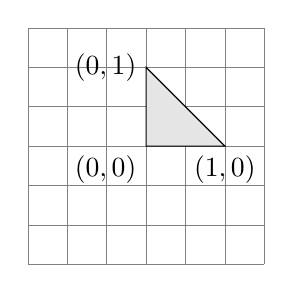
\begin{tikzpicture}[scale=0.5]
            \draw[step=1cm,gray,very thin] (-3,-3) grid (3,3);
            \filldraw[fill=gray!20, draw=black] (0,0) -- (2,0) -- (0,2) -- cycle;
            \node at (0,0) [below left] {$(0,0)$};
            \node at (2,0) [below] {$(1,0)$};
            \node at (0,2) [left] {$(0,1)$};
        \end{tikzpicture}
        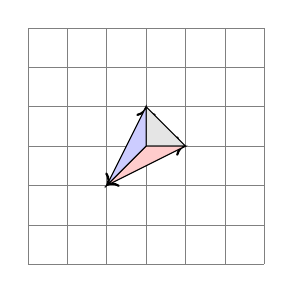
\begin{tikzpicture}[scale=0.5]
            \draw[step=1cm,gray,very thin] (-3,-3) grid (3,3);
            \draw[thick,->] (0,0) -- (1,0);
            \draw[thick,->] (0,0) -- (0,1);
            \draw[thick,->] (0,0) -- (-1,-1);
            % fill in the upper right quadrant
            \filldraw[fill=gray!20, draw=black] (0,0) -- (1,0) -- (0,1) -- cycle;
            % fill in the region from pi/2 to 5pi/4 
            \filldraw[fill=red!20, draw=black] (0,0) -- (-1,-1) -- (1,0) -- cycle;
            % fill in the region from 5pi/4 to 3pi/2
            \filldraw[fill=blue!20, draw=black] (0,0) -- (-1,-1) -- (0,1) -- cycle;
        \end{tikzpicture}
    \end{center} 
    Note that the fan has three 2-dimensional cones which are filled in.
    These cones represent the three standard coordinate charts of $\P^2$ given by
    $x_i \neq 0$ for $i = 0,1,2$. The isosceles right triangle with
    side lenghth $a$ corresponds to the $a$-th Veronese 
    embedding of $\P^2$.
\end{example}
Fans are more friendly objects for algebraic geometers and 
one can read further about them in \cite{cls}. The data of a fan,
and in particular the primitive edge vectors (defined as the generators of the rays of the fan),
will prove important in our discussion on equivariant cohomology.

\subsection{Prequantization}
Manifolds equipped with integral symplectic forms admit prequantization line bundles.
In particular we have the following theorem. 

\begin{theorem}
    Let $(M,\omega)$ be a symplectic manifold. Suppose that $[\omega]$ is integral. Then 
    there exists a "prequantization" line bundle $\cL \to M$ with $c_1(\cL) = [\omega]$ and a Hermitian connection $\alpha$
    whose corresponding curvature form is $\omega$. Moreover $\cL$ is unique up to isomorphism 
    (but still requires a particular choice). 
\end{theorem}

\begin{remark}
    \red{I don't quite understand the so-what of this theorem. What comes after "prequantization"?}
\end{remark}

\begin{proposition}
    The line bundle $\cL = U \times_{K_C} \C$ where $K_\C$ acts on $\C$ with 
    weight $\nu = L(-\lambda)$ is a prequantization line bundle for $M = U/K_\C$. Note that $\nu \in k^*$ is the 
    dual Lie algebra of $K_\C$.
\end{proposition}
\begin{proof}
    See \cite{hamilton}.
\end{proof}
Symplectic reduction realizes a Kahler form on the reduced space, in particular
$M$ and $\cL$ actually carry complex structures. The following theorem is about the space of
holomorphic sections of $\cL$.
\begin{theorem}
    With the setup above, we have \begin{align*}
        \dim H^0(M,\cL) = \#(\text{integer points in } P)
    \end{align*}
\end{theorem}

\begin{proof}
    A holomorphic section of $\cL$ over $M$ corresponds to a $K_\C$-equivariant holomorphic function $f:U\to \C$. 
    Such $f$ extends to all of $\C^N$ because of Hartog's theorem (A holomorphic function on $\C^N$ for $N>1$ canont have 
    an isolated singularity and therefore cannot have a singularity on a submanifold of codimension $\geq 2$).

    \hfill

    Write such a function as its Taylor series so that \begin{align*}
        f = \sum_{\alpha\in\N^n} c_\alpha z^\alpha
    \end{align*} Consider the equivariance one term at a time. 
    Thinking about the monomial $f(z) = z^I$ we 
    see that \begin{align*}
        f(k\cdot z) &= f(i(k)\cdot z) = (i(k)\cdot z)^I = i(k)^Iz^I = k^{i^*(I)}z^I \\
        k\cdot f(z) &= k^{\nu}z^I
    \end{align*} and therefore a basis for the space of equivariant functions $f:U\to \C$ 
    is given by the monomials corresponding to lattice points in $P$.
\end{proof}



\section{Equivariant cohomology}
We introduce equivariant cohomology and some classical results about the
$T$-equivariant cohomology of smooth projective toric varieties.

\subsection{Basic properties}
Let $G$ be a Lie group. The equivariant cohomology ring $H_G^*(X)$ of a $G$-space $X$ is
defined as the singular cohomology of the Borel construction $X\times_G EG$,
where $EG$ is a contractible space on which $G$ acts freely. Such a space
always exists and is unique up to homotopy equivalence \cite{hatcher}.

\hfill

Here are some important properties to know about equivariant cohomology:

\begin{enumerate}
	\item functoriality;
	\item a ring structure;
	\item excision;
	\item the Mayer-Vietoris sequence;
	\item the Künneth formula;
	\item the Leray spectral sequence;
	\item for smooth orientable $X$, Poincaré duality; and
	\item existence of Chern classes,
\end{enumerate}
where all subsets and maps are assumed to be equivariant. The
ring $H^*_T(X)$ is a module over $H^*_T(\text{pt})$ via the map $X \to \text{pt}$.

\hfill

We now introduce a notion of equivariant formality which is a particularly
nice algebraic notion.
It implies that
the equivariant cohomology of $X$ is a free module over the equivariant cohomology
of a point.

\begin{definition}
	A $G$-space $X$ is called \textbf{equivariantly formal} if the Leray spectral sequence
	associated to the fibration $X \to X \times_T ET \to BT$ collapses at the $E_2$-page.
\end{definition}

By definition, we have that
\begin{proposition}
	If $X$ is equivariantly formal, then \begin{align*}
		H^*_G(X) \cong H^*_G(\text{pt}) \otimes H^*(X).
	\end{align*}
\end{proposition}

When $X$ is equivariantly formal,
the ordinary cohomology can be recovered from
equivariant cohomology as the quotient
\[
	H^*(X) = \frac{H^*_T(X)}{M \cdot H^*_T(X)}
\]
which in effect simply sets each $t_i = 0$.
In particular, $H^*_T(X)$ is a free module over $H^*_T(\text{pt})$.

\hfill

Many varieties of interest are equivariantly formal, such as all of the following:
\begin{enumerate}
	\item a smooth complex projective variety (with respect to any linear algebraic $T$-action);
	\item a variety whose ordinary cohomology vanishes in odd degree (with respect to any $T$-action);
	\item a compact symplectic manifold with a Hamiltonian $T$-action, where $T$ is a compact torus.
\end{enumerate}
See \cite{fulton-anderson} for a good discussion of these facts.

\subsection{Examples}
We introduce some examples.

\begin{example}
	We can identify $U(n)$ as those complex matrices preserving
	the standard Hermitian form on $\C^n$. The group $U(n)$ acts on $S^{2n-1}$ transitively
	and the stabilizer of the point $(1,0,\ldots,0)$ is $U(n-1)$.

	Therefore there is a canonical action of $U(1)$ acting as scalar matrices on $S^{2n-1}$
	inherited from the action on $U(n)$. None of these odd dimensional spheres are contractible,
	but $S^\infty$ is contractible. In particular $EU(1) = S^\infty$ and \begin{align*}
		BU(1) = S^\infty/U(1) = \C\P^\infty
	\end{align*}
	Therefore \begin{align*}
		H^*_{U(1)}(pt) = H^*(\C\P^\infty) = \Z[t]
	\end{align*} where $t$ is the first Chern class of the tautological line bundle and $\deg t = 2$.
\end{example}

\begin{example}
	In general, $H_T^*(pt)$ can be identified with the representation ring of $T$. \begin{align*}
		BT \cong \prod_{\rank T} \C\P^\infty
	\end{align*}

	Given a representation $V$ of $T$,
	we can form a vector bundle on the classifying space whose
	total Chern class is equal to the class of $V$ in the representation ring, c.f. \cite{huybrechts}.
\end{example}
\subsection{Danilov's theorem}
The geometry of a smooth projective toric variety $X$ is particularly special because
it is encoded in the combinatorics of the fan of $X$.
Danilov's theorem gives a presentation of the ordinary cohomology ring of $X$ in terms of the
combinatorics of the fan of $X$.
\begin{theorem}\label{thm:danilov}
	[Danilov]
	Let $X$ be a smooth projective toric variety. Then the ordinary cohomology ring
	of $X$ is \begin{align*}
		H^*(X)\cong \Q[\alpha_1,\ldots,\alpha_n]/(I+J)
	\end{align*} where $I$ is the ideal generated by the linear relations among the
	$\alpha_i$
	\begin{align*}
		\sum_{i=1}^n \langle v_i,u\rangle \alpha_i \in I
	\end{align*} for $u\in M$ and $v_1,\ldots,v_n$ the fundamental
	vectors of the rays of the fan of $X$,
	and $J$ is the ideal generated by the Stanley-Reisner relations. \begin{align*}
		\alpha_{i_1}\cdots\alpha_{i_k}\in J \text{ if } \{i_1,\ldots,i_k\} \text{ is not a cone of the fan of } X.
	\end{align*}
\end{theorem}

Danilov's original proof of the theorem is quite involved and invokes
a lot of intersection theory, but using facts from equivariant cohomology
and toric geometry, we can give a much simpler proof. In particular
smooth projective toric varieties are equivariantly formal. The proof of theorem
\ref{thm:danilov} will be deferrred to the next section where we
introduce the localization theorem. It is a good example of how the theory of equivariant
cohomology enriches ordinary cohomology.

\subsection{ABBV localization}
At its core, the ABBV localization formula arises from the principle that,
under certain conditions, integrals over a compact space with a torus action can be “localized”
to the fixed points of the action. This idea can be traced back to the stationary
phase approximation in physics, where integrals are approximated by contributions
from critical points. In the equivariant cohomology setting, the fixed points of the torus action play a similar role.
\begin{theorem}
	[Atiyah-Bott, Berline-Vergne] Suppose a torus $T$ of dimensionl $l$ acts on a
	compact oriented manifold $M$ with fixed point set $F$. If $\phi \in H^*_T(M)$, then
	\begin{align*}
		\int_M \phi = \sum_{x\in F} \frac{i^*_x\phi}{e_x}
	\end{align*} where $e_x$ is the equivariant Euler class of the normal bundle of $x$ in $M$.
\end{theorem}
In particular, we will apply this theorem when the fixed point set is a finite set of points,
in which case the localization formula becomes \begin{align*}
	\int_M \phi = \sum_{x\in F} \frac{\phi(x)}{e_x}
\end{align*} where $e_x$ is the equivariant Euler class of $T_xM$. In particular, $e_x$
is the product of the weights of the action of $T$ on $T_xM$. Moreover, the weights are
distinct because the fixed point set is isolated.

\hfill 

We will now consider the localization theorem in an example.
In general, \cite{tu} contains a proof of the ABBV localization formula 
for $S^1$-actions.

\begin{example}
    Consider the two sphere $S^2$ with real coordinates $(x,y,z)$ and the $S^1$-action \begin{align*}
        e^{i\theta}\cdot(x,y,z) = (x\cos\theta - y\sin\theta, x\sin\theta + y\cos\theta, z).
    \end{align*}
    which rotates the sphere about the $z$-axis. The fixed points of this action are the north and south poles.

    \hfill 

    The Cartan model of equivariant cohomology suggests that we can consider integrating an equivariant cohomology
    class over $S^2$ by integrating corresponding \emph{equivariant differential forms} over $S^2$. In particular
    if we consider the equivariant symplectic form $\alpha = \omega + 2\pi\mu$ where $\mu(x,y,z) = z$
    is the moment map, viewed as a degree $0$ form. $\alpha$ is equivariantly closed because
    in the Cartan model, the equivariant differential is given by \begin{align*}
        d_X = d - ui_X
    \end{align*} where $i_X$ is the contraction with the vector field $X$ generating the $S^1$-action
    and $u$ is the standard representation of $S^1$, the "equivariant parameter". 

    Therefore $\alpha$ represents a class in $H^2_{S^1}(S^2)$. We can compute the integral of $\alpha$ over $S^2$ 
    using the localization formula. \begin{align*}
        \int_{S^2} \alpha &= \frac{\mu(N)}{\text{weight of $U(1)$ action on $T_N S^2$}} 
        + \frac{\mu(S)}{\text{weight of $U(1)$ action on $T_S S^2$}} \\
        &= 2\pi\mu(N) - 2\pi\mu(S) = 4\pi
    \end{align*} where $N$ and $S$ are the north and south poles respectively. Indeed
    the surface area of $S^2$ is $4\pi$.
\end{example}

\subsection{Proof of Danilov's theorem}
\subsubsection{Cone-orbit correspondence}
Let $T$ be an $n$-dimensional torus with character group $M$. Let $N = \Hom(M,\Z)$ be the
dual lattice, their pairing is denoted by $\langle \cdot,\cdot\rangle$. Let $X = X(\Sigma)$ be a smooth
complete toric variety, which are in bijection with complete nonsingular fans $\Sigma$ in $N_\R$.

\hfill

For any convex cone $\sigma \subset N_\R$, the \emph{dual cone} in $M_\R$ is \begin{align*}
    \sigma^\vee = \{u\in M_\R \mid \langle u,v\rangle \geq 0 \text{ for all } v\in \sigma\}.
\end{align*} By intersecting with the lattice, we obtain a semigroup $\sigma^\vee \cap M$
with corresponding semigroup algebra $\C[\sigma^\vee \cap M]$. The toric variety $X$
is covered by $T$-variant open affine sets \begin{align*}
    U_\sigma = \Spec \C[\sigma^\vee \cap M]
\end{align*} The affine charts corresponding to the top-dimensional cones of $\Sigma$ 
are enough to cover $X$, and the intersection of cones corresponds to the intersection of
affine charts.

\hfill

Each cone $\tau$ of the fan also defines a torus-invariant subvariety $V(\tau)$ of $X$ of codimension $\dim \tau$.
On open affines, the subvariety looks like \begin{align*}
    V(\tau) \cap U_\sigma = \Spec \C[\tau^{\perp} \cap \sigma^\vee \cap M] \hookrightarrow \Spec \C[\sigma^\vee \cap M]
\end{align*} and so elements of the dual lattice $N$ can be thought of as rational functions on $X$.
\subsubsection{Bialynicki-Birula decomposition}
The Bialynicki-Birula decomposition is a 
generalization of the Morse theory for torus actions. Suppose 
that $\C^*$ acts on a smooth projective variety $X$ with finitely 
many fixed points $p_1,\ldots,p_k$. 

\hfill

Then each $T_{p_i}X$ is a representation of $\C^*$, and so we can decompose
into weight spaces \begin{align*}
    T_{p_i}X = \bigoplus_{\lambda\in \C} V_\lambda
\end{align*} where $V_\lambda = \set{v\in T_{p_i}X \mid t\cdot v = t^\lambda v}$.
Note that $\lambda\neq 0 $ because the fixed point set is isolated.

Define the attracting set \begin{align*}
    C_i = \set{x\in X \mid \lim_{t\to 0} t\cdot x = p_i}
\end{align*} 

\begin{theorem}
    [Bialynicki-Birula] 
    There existsa filtration of $X$ by closed subschemes \begin{align*}
        X = X_n \supset X_{n-1} \supset \cdots \supset X_0 
    \end{align*} such that 
    each $X_i \backslash X_{i-1}$ is a disjoint union of affine spaces called cells, 
    in particular the attracting sets.
\end{theorem}

\begin{cor}
    Let $X$ as above. Then \begin{enumerate}
        \item $H_{2i+1}(X) = 0$ for all $i$;
        \item $H_{2i}(X)$ is a $\Z$-module freely generateed by the classes
        of the closures of the $i$-dimensional cells.
    \end{enumerate}
\end{cor}

\subsubsection{Shellings}
In this section, we apply the setup 
of the Bialynicki-Birula decomposition to the context of toric varieties.

\hfill

Let $X = X(\Sigma)$ be projective, with $P$ 
a polytope whose normal fan is $\Sigma$. Choosing
a general vector $v\in N_\R$ we obtain an ordering of the vertices 
$u_1,\ldots,u_s$ of $P$ by the order of the inner products $\langle v,u_i\rangle$.
Geometrically, we are choosing a $1$-parameter subgroup of the torus $T$ 
which acts on $X$. The correpsonding sub-moment map turns out to be
a perfect Morse-Bott function on $X$.

\hfill

By the polytope-fan correspondence,
we get an ordering of the maximal cones $\sigma_1,\ldots,\sigma_s$ of $\Sigma$.
For $1\leq i \leq s$ let \begin{align*}
    \tau_i = \bigcap_{j>i, \dim(\sigma_j \cap \sigma_i) = n-1} \sigma_j \cap \sigma_i
\end{align*} so that 
$\tau_1 = \set{0}, \tau_s = \sigma_s$ and $\tau_p \subset \tau_q$
implies $p \leq q$. Such an ordering of cones 
is called a \emph{shelling} of $\Sigma$. 

\begin{proposition}
    A shelling gives a cellular decomposition of $X$, with
the closures of the cells being $V(\tau_i)$. In particular,
the classes \begin{align*}
    \alpha_i = [V(\tau_i)] \in H^{2(n-\dim \tau_i)}(X)
\end{align*}
form an additive $\Z$-basis of $H^*(X)$.
\end{proposition}


The $V(\tau_i)$ are precisely the closures of the attracting sets 
of the chosen $\C^*$-action on $X$. We will demonstrate this in a particularly
pleasant example.
\begin{example}
    [Morse theory on $\C\P^2$]
    Classically, recall that the Chow ring (or cohomology ring) of
     $\C\P^2$ is \begin{align*}
        H^*(\C\P^2) = \Z[0] \oplus \Z[\P^1] \oplus \Z[\P^2]
    \end{align*} Consider the standard action of $T^2$ on $\C\P^2$
    and consider the $1$-parameter subgroup acting by $t\cdot[x:y:z] = [tx:t^2y:z]$.
    Consider the following moment image, whose 
    edges are labled by the weights of the action on the tangent space at the fixed points:
    
\end{example}


\subsection{GKM Theory}


\section{Appendix A: Vector bundles and connections}
We provide a brief introduction to connections on vector bundles.
\subsection{Parallel transport}
One way to think about a connection is to consider parallel transport. You want to 
be able to differentiate sections of a vector bundle along paths. When we are dealing with functions,
we can form the directional derivative  \begin{align*}
    ds(x)X = \lim_{t\to 0}\frac{s(\gamma(t)) - s(\gamma(0))}{t}
\end{align*} for any smooth path $\gamma$ representing the tangent vector $X\in T_xM$ 
and this expression gives us a linear map $ds(x):T_xM\to E_x$.

However if $E$ is a nontrivial bundle, then this expression does not make sense because the
 summands live in different fibers. There is unfortunately no natural way to 
 compare vectors in different fibers. Therefore we need to introduce additional structure to 
 be able to compare these fibers.

For a general vector bundle $E\to M$, we want to associate, to a path $\gamma$ in $M$, a smooth family of 
parallel transport isomorphisms $P^t_\gamma: E_{\gamma(0)}\to E_{\gamma(t)}$ such that \begin{itemize}
    \item $P^0_\gamma = \id$
    \item $P^t_{\gamma_1\cdot\gamma_2} = P^t_{\gamma_2}\circ P^t_{\gamma_1}$
\end{itemize} for any paths $\gamma_1,\gamma_2$ and $t\in\R$.


Such a choice would allow us to define the directional ("covariant") derivative of a section $s$ along a path $\gamma$ 
as before. We shuold require that \begin{itemize}
    \item The directional derivative depends only on $s$ and $X\in T_xM$, not the particular 
    choice of $\gamma$.
    \item The map $\nabla s(x):T_xM\to E_x$ is $\C$-linear.
\end{itemize}
This will give us the richest notion of a connection on a vector bundle.
\subsection{Connections}
In this section, we consider $M$ a real manifold and $\pi:E\to M$ complex vector bundle.
Let $\cA^i(E) = \Omega^i(M) \otimes E$ denote the sheaf of smooth $i$-forms with values in $E$.
\begin{definition}
    A \textbf{connection} on $E$ 
    is a $\C$-linear map of sheaves
    $\nabla:\cA^0(E)\to\cA^1(E)$ satisfying the Leibniz rule
    \begin{align*}
        \nabla(fs) = df\otimes s + f\nabla s
    \end{align*}
\end{definition}
We can interpret this definition in the sense of parallel transport. Given 
a section $s\in\cA^0(E)$, we can differentiate it along a path $\gamma$ to get another 
section of $E$, i.e. $\nabla:\Gamma(E)\to \Gamma(\Hom(TM,E))$.
\begin{theorem}
    The space of all connections $\cA(E)$ is an affine space modelled on $\cA^1(\End E)$. In particular \begin{itemize}
        \item $\cA(E)$ is nonempty
        \item For any two connections $\nabla_1,\nabla_2$ the difference $\nabla_1-\nabla_2$ 
        is a global section of $\cA^1(\End E)$.
        \item $(\nabla + a)s := \nabla s + as$ is a connection whenever $\nabla$ is a connection and 
        $a\in\cA^1(\End E)$.
    \end{itemize}
\end{theorem}
\begin{proof}
    See \cite{huybrechts}.
\end{proof}
The idea of a connection generalizes the exterior differential to sections of general vector bundles. 
However, a connection need not satisfy $\nabla^2 = 0$ in general. The obstruction for a connection
define a differential is measured by its curvature. We explain this now.

\subsection{Curvature}

A connection $\nabla:\cA^0(E)\to \cA^1(E)$ induces "differentials" \begin{align*}
    \nabla:\cA^i(E)\to\cA^{i+1}(E)
\end{align*} given by the formula \begin{align*}
    \nabla(\alpha\otimes s) = d\alpha\otimes s + (-1)^i\alpha\wedge\nabla s
\end{align*}

\begin{definition}
    The \textbf{curvature} $F_\nabla$ of a connection $\nabla$ is the composition \begin{align*}
        F_\nabla := \nabla^2:\cA^0(E)\to\cA^2(E)
    \end{align*} In particular $F_\nabla$ is a global section of $\cA^2(\End E)$. This is because 
    the curvature homomorphism is $\cA^0$-linear.
\end{definition}

\begin{example}
    Consider the connections on the trivial bundle $M\times \C^r$. If $\nabla = d$ is the
    trivial connection then $F_\nabla = 0$. 

    Any other connection is of the form $\nabla = d + A$ where $A$ is a matrix of 1-forms. For a section
    $s$ we compute \begin{align*}
        F_\nabla(s) &= (d+A)(d+A)(s) \\
        &= d^2s + dAs + Ads + AAs \\
        &= d(A)s + A\wedge As
    \end{align*} and therefore \begin{align*}
        F_\nabla = dA + A\wedge A
    \end{align*}
    For line bundles we get that $F_\nabla = dA$ is an ordinary 2-form.
\end{example}

\section{Appendix B: Prequantization}
Manifolds equipped with integral symplectic forms admit prequantization line bundles in the following sense, cf. \cite{lsg}:

\begin{theorem}
    Let $(M,\omega)$ be a symplectic manifold. Suppose that $[\omega]$ is integral. Then 
    there exists a "prequantization" line bundle $\cL \to M$ with $c_1(\cL) = [\omega]$ and a Hermitian connection $\alpha$
    whose corresponding curvature form is $\omega$. Moreover $\cL$ is unique up to isomorphism.
\end{theorem}

Let $P$ be a Delzant polytope. Complexifying (\ref{eq:ses1}) and passing to the dual of the Lie algebras, we get \begin{align*}
    1\to K_\C \to T_\C^N \to T_\C^n \to 1 \\
    0 \to (\R^n)^* \to (\R^N)^* \to k^* \to 0
\end{align*} where $k^*$ is the dual of the Lie algebra of $K_\C$. 
Let $F_i$ denote the facets of $\Delta$ and for any $z = (z_1,\dots,z_N)\in\C^n$ let $F_z := \cap_{z_i = 0}F_i$.
Consider the set \begin{align*}
    U = \{z\in\C^n: F_z \neq \emptyset\}
\end{align*} Recall that we defined the toric symplectic manifold $X_2(P) = U/K_\C$.

\begin{proposition}
    The line bundle $\cL = U \times_{K_C} \C$ where $K_\C$ acts on $\C$ with 
    weight $\nu = i^*(-\lambda)$ is a prequantization line bundle for $M = U/K_\C$. 
\end{proposition}

Symplectic reduction realizes a Kahler form on the reduced space, in particular
$M$ and $\cL$ actually carry complex structures. The following theorem is about the space of
holomorphic sections of $\cL$.
\begin{theorem}
    With the setup above, we have \begin{align*}
        \dim H^0(M,\cL) = \#(\text{integer points in } P)
    \end{align*}
\end{theorem}

\begin{proof}
    A holomorphic section of $\cL$ over $M$ corresponds to a $K_\C$-equivariant holomorphic function $f:U\to \C$. 
    Such $f$ extends to all of $\C^N$ because of Hartog's theorem (A holomorphic function on $\C^N$ for $N>1$ canont have 
    an isolated singularity and therefore cannot have a singularity on a submanifold of codimension $\geq 2$).

    Write such a function as its Taylor series so that \begin{align*}
        f = \sum_{\alpha\in\N^n} c_\alpha z^\alpha
    \end{align*} Consider the equivariance one term at a time. 
    Thinking about the monomial $f(z) = z^I$ we 
    see that \begin{align*}
        f(k\cdot z) &= f(i(k)\cdot z) = (i(k)\cdot z)^I = i(k)^Iz^I = k^{i^*(I)}z^I \\
        k\cdot f(z) &= k^{\nu}z^I
    \end{align*} and therefore a basis for the space of equivariant functions $f:U\to \C$ 
    is given by \begin{align*}
        \set{z^I \st i^*(I) = \nu, I\in\N^n}
    \end{align*} and the set of such $I$ is \begin{align*}
        \Z^n_+ \cap (i^*)^{-1}(\nu)
    \end{align*} monomials corresponding to lattice points in $P$.
\end{proof}



\bibliography{refs}{}
\bibliographystyle{plain}


\end{document}